\documentclass[12pt]{article}
\usepackage{amsfonts,amssymb,float,amsmath}
\usepackage{algorithmic}
\usepackage{graphicx, siunintx}
\usepackage{textcomp}
\usepackage{xcolor}
\usepackage{txfonts}
\usepackage{multicol}
\usepackage{listings}
\usepackage{enumitem}
\usepackage{mathtools}
\usepackage{gensymb}
\usepackage{comment}
\usepackage[breaklinks=true]{hyperref}
\usepackage{tkz-euclide} 
\usepackage{listings}
\usepackage{gvv}                       
\usepackage{gvv-book}
%\def\inputGnumericTable{}                             
\usepackage{color}                                            
\usepackage{array}                                            
\usepackage{longtable}                                       
\usepackage{calc}                                             
\usepackage{multirow}                                         
\usepackage{hhline}                                           
\usepackage{ifthen}                                           
\usepackage{lscape}
\newcommand{\BEQA}{\begin{eqnarray}}
\newcommand{\EEQA}{\end{eqnarray}}
%\newcommand{\define}{\stackrel{\triangle}{=}}
\theoremstyle{remark}
\newtheorem{rem}{Remark}
\parindent 0px
\pagenumbering{gobble}
\begin{document}
\title{\vspace{-5cm}Gate paper 2023-XH}
\author{Ayush Sunil Labhade}
\date{AI25Btech11002}
\maketitle

\begin{flushright}Humanities and Social Sciences – Sociology (XH-C6)\end{flushright}
\begin{flushleft}General Aptitude \textbf{\brak{GA}} \\[5pt]
\textbf{\item Q.1 – Q.5 Carry ONE mark Each}\end{flushleft}
\begin{enumerate}
%Q.1
\item Rafi told Mary, “I am thinking of watching a film this weekend.”
The following reports the above statement in indirect speech: 
Rafi told Mary that he \_\_\_\_\_\_\_ of watching a film that weekend.
\begin{enumerate}
    \begin{multicols}{2}
        \item thought
        \item is thinking
        \item am thinking
        \item was thinking
    \end{multicols}
\end{enumerate}
\hfill\brak{GATE \ XH \ 2023}
%Q.2
\item Permit : \_\_\_\_\_\_\_ : : Enforce : Relax 
\brak{By word meaning}
\begin{enumerate}
    \begin{multicols}{4}
        \item Allow
        \item Forbid
        \item License
        \item Reinforce
    \end{multicols}
\end{enumerate}
\hfill\brak{GATE \ XH \ 2023}
%Q.3
\item Given a fair six-faced dice where the faces are labelled ‘1’, ‘2’, ‘3’, ‘4’, ‘5’, and ‘6’, 
what is the probability of getting a ‘1’ on the first roll of the dice and a ‘4’ on the 
second roll?
\begin{enumerate}
    \begin{multicols}{4}
        \item $\frac{1}{36}$
        \item $\frac{1}{6}$
        \item $\frac{5}{6}$
        \item $\frac{1}{3}$
    \end{multicols}
\end{enumerate}
\hfill\brak{GATE \ XH \ 2023}
%Q.4
\item A recent survey shows that 65% of tobacco users were advised to stop consuming tobacco.
The survey also shows that 3 out of 10 tobacco users attempted to stop using tobacco.
Based only on the information in the above passage, which one of the following options can be logically inferred with certainty?
\begin{enumerate}
    \item A majority of tobacco users who were advised to stop consuming tobacco made an attempt to do so.
    \item A majority of tobacco users who were advised to stop consuming tobacco did not attempt to do so.
    \item Approximately 30% of tobacco users successfully stopped consuming tobacco.
    \item Approximately 65% of tobacco users successfully stopped consuming tobacco.
\end{enumerate}
\hfill\brak{GATE \ XH \ 2023}
%Q.5
\item How many triangles are present in the given figure?
\begin{figure}[H]
    \centering
    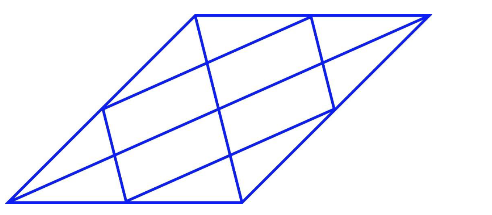
\includegraphics[width=0.5\textwidth]{Figs/Q5.png}
    \caption{}
    \label{fig:6.1}
\end{figure}
\begin{enumerate}
    \begin{multicols}{4}
        \item 12
        \item 16
        \item 20
        \item 24
    \end{multicols}
\end{enumerate}
\hfill\brak{GATE \ XH \ 2023}
\newpage
\textbf{Q.6 – Q.10 Carry TWO marks Each}
%Q.6
\item Students of all the departments of a college who have successfully completed the registration process are eligible to vote in the upcoming college elections. However, by the time the due date for registration was over, it was found that surprisingly none of the students from the Department of Human Sciences had completed the registration process. Based only on the information provided above, which one of the following sets of statement(s) can be logically inferred with certainty?
\begin{enumerate}
    \item[(i)] All those students who would not be eligible to vote in the college elections would certainly belong to the Department of Human Sciences.
    \item[(ii)] None of the students from departments other than Human Sciences failed to complete the registration process within the due time.
    \item[(iii)] All the eligible voters would certainly be students who are not from the Department of Human Sciences.
\end{enumerate}
\begin{enumerate}
    \begin{multicols}{4}
        \item (i) and (ii)
        \item (i) and (iii)
        \item only (i)
        \item only (iii)
    \end{multicols}
\end{enumerate}
\hfill\brak{GATE \ XH \ 2023}
%Q.7
\item Which one of the following options represents the given graph?
\begin{figure}[H]
    \centering
    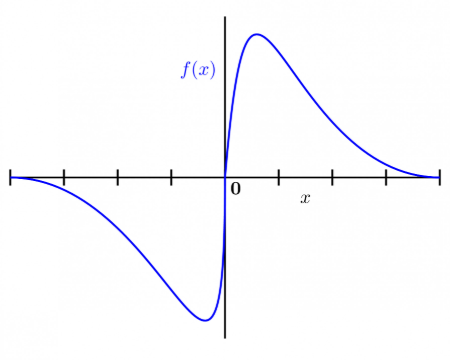
\includegraphics[width=0.6\textwidth]{Figs/Q7.png}
    \caption{}
    \label{fig:6.2}
\end{figure}
\begin{enumerate}
    \begin{multicols}{4}
        \item $f(x)=x^22^{-|x|}$ 
        \item $f(x)=x2^{-|x|}$
        \item $f(x)=|x|2^{-x}$ 
        \item $f(x)=x2^{-x}$
    \end{multicols}
\end{enumerate}
\hfill\brak{GATE \ XH \ 2023}
%Q.8
\item Which one of the options does NOT describe the passage below or follow from it?
We tend to think of cancer as a ‘modern’ illness because its metaphors are so modern. It is a disease of overproduction, of sudden growth, a growth that is unstoppable, tipped into the abyss of no control. Modern cell biology encourages us to imagine the cell as a molecular machine. Cancer is that machine unable to quench its initial command \brak{to grow} and thus transform into an indestructible, self-propelled automaton.
\sbrak{Adapted from \textit{The Emperor of All Maladies} by Siddhartha Mukherjee}
\begin{enumerate}
    \item It is a reflection of why cancer seems so modern to most of us.
    \item It tells us that modern cell biology uses and promotes metaphors of machinery.
    \item Modern cell biology encourages metaphors of machinery, and cancer is often imagined as a machine.
    \item Modern cell biology never uses figurative language, such as metaphors, to describe or explain anything.
\end{enumerate}
\hfill\brak{GATE \ XH \ 2023}
%Q.9
\item The digit in the unit’s place of the product $3^{999} \times 7^{1000}$ is \_\_\_\_\_\_\_.
\begin{enumerate}
    \begin{multicols}{4}
        \item 7
        \item 1
        \item 3
        \item 9
    \end{multicols}
\end{enumerate}
\hfill\brak{GATE \ XH \ 2023}
%Q.10
\item A square with sides of length 6 cm is given. The boundary of the shaded region is defined by two semi-circles whose diameters are the sides of the square, as shown. The area of the shaded region is \_\_\_\_\_\_\_ cm$^2$.
\begin{figure}[H]
    \centering
    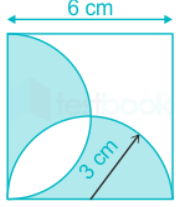
\includegraphics[width=0.3\textwidth]{Figs/Q10.png}
    \caption{}
    \label{fig:6.3}
\end{figure}
\begin{enumerate}
    \begin{multicols}{4}
        \item $6\pi$
        \item 18
        \item 20
        \item $9\pi$
    \end{multicols}
\end{enumerate}
\hfill\brak{GATE \ XH \ 2023}
\newpage
\textbf{Reasoning and Comprehension (XH-B1)\newline XH-B1: Q.11 – Q.17 Carry ONE mark Each}
%Q.11
\item Which word below best describes the idea of being both Spineless and Cowardly?
\begin{enumerate}
    \begin{multicols}{2}
        \item Pusillanimous
        \item Unctuous
        \item Obsequious
        \item Reticent
    \end{multicols}
\end{enumerate}
\hfill\brak{GATE \ XH \ 2023}
%Q.12
\item Choose the right preposition to fill up the blank: The whole family got together \_\_\_\_\_\_\_ Diwali
\begin{enumerate}
    \begin{multicols}{4}
        \item of
        \item at
        \item in
        \item till
    \end{multicols}
\end{enumerate}
\hfill\brak{GATE \ XH \ 2023}
%Q.13
\item Select the correct option to fill in all the blanks to complete the passage:
The (i)\_\_\_\_\_\_\_ factor amid this turbulence has been the (ii)\_\_\_\_\_\_\_\_ of high
octane, action-oriented films such as RRR, K.G.F: Chapter 2 and Pushpa from film
industries in the south of the country. Traditionally, films made in the south have
done well in their own (iii) \_\_\_\_\_\_\_\_\_. But increasingly, their dubbed versions
have performed well in the Hindi heartland, with collections (iv)\_\_\_\_\_\_\_\_ those of
their Bollywood counterparts.
\begin{enumerate} 
\item (i) disheartening (ii) failure (iii) channels (iv) matching
\item (i) redeeming (ii) outperformance (iii) geographies (iv) eclipsing
\item (i) shocking (ii) underperformance (iii) cinemas (iv) below
\item (i) humbling (ii) bombing (iii) theatres (iv) falling behind
\end{enumerate}
\hfill\brak{GATE \ XH \ 2023}
%Q.14
\item The following passage consists of 6 sentences. The first and sixth sentences of the
passage are at their correct positions, while the middle four sentences (represented
by 2, 3, 4, and 5) are jumbled up. Choose the correct sequence of the sentences so that they form a coherent
paragraph:
\begin{enumerate}
\item[1.] Most obviously, mobility is taken to be a geographical as well as a social phenomenon.
\item[2.] Much of the social mobility literature regarded society as a uniform surface and failed to register the geographical intersections of region, city and place, with the social categories of class, gender and ethnicity.
\item[3.] The existing sociology of migration is incidentally far too limited in its concerns to be very useful here.
\item[4.] Further, I am concerned with the flows of people within, but especially beyond, the territory of each society, and how these flows may relate to many different desires, for work, housing, leisure, religion, family relationships, criminal gain, asylum seeking and so on.
\item[5.] Moreover, not only people are mobile but so too are many ‘objects’.
\item[6.] I show that sociology’s recent development of a ‘sociology of objects’ needs to be taken further and that the diverse flows of objects across societal borders and their intersections with the multiple flows of people are hugely significant.
\end{enumerate}
\begin{enumerate}
    \begin{multicols}{4}
        \item 3, 2, 5, 4
        \item 2, 3, 4, 5
        \item 5, 4, 3, 2
        \item 4, 2, 5, 3
    \end{multicols}
\end{enumerate}
\hfill\brak{GATE \ XH \ 2023}
%Q.15
\item The population of a country increased by 5\% from 2020 to 2021. Then, the
population decreased by 5\% from 2021 to 2022. By what percentage did the
population change from 2020 to 2022?
\begin{enumerate}
    \begin{multicols}{4}
        \item -0.25\%
        \item 0\%
        \item 2.5\%
        \item 10.25\%
    \end{multicols}
\end{enumerate}
\hfill\brak{GATE \ XH \ 2023}
%Q.16
\item The words \textbf{Thin: Slim: Slender} are related in some way.
Identify the correct option(s) that reflect(s) the same relationship:
\begin{enumerate}
    \begin{multicols}{2}
        \item Fat: Plump: Voluptuous
        \item Short: Small: Petite
        \item Tall: Taller: Tallest
        \item Fair: Dark: Wheatish
    \end{multicols}
\end{enumerate}
\hfill\brak{GATE \ XH \ 2023}
%Q.17
\item A pandemic like situation hit the country last year, resulting in loss of human life and economic depression. To improve the condition of its citizens, the government made a series of emergency medical interventions and increased spending to revive the economy. In both these efforts, district administration authorities were actively involved. Which of the following action(s) are plausible?
\begin{enumerate}
    \item In future, the government can make district administration authorities responsible for protecting health of citizens and reviving the economy.
    \item The government may set up a task force to review the post pandemic situation and ascertain the effectiveness of the measures taken.
    \item The government may set up a committee to formulate a pandemic management program to minimize losses to life and economy in future.
    \item The government may take population control measures to minimize pandemic related losses in future.
\end{enumerate}
\hfill\brak{GATE \ XH \ 2023}
\newpage
\textbf{XH-B1: Q.18 – Q.26 Carry TWO marks Each}
%Q.18
\item Six students, Arif, Balwinder, Chintu, David, Emon and Fulmoni appeared in the GATE-XH exam in 2022. Balwinder scores less than Chintu in XH-B1, but more than Arif in XH-C1. David scores more than Balwinder in XH-C1, and more than Chintu in XH-B1. Emon scores less than David, but more than Fulmoni in XH-B1. Fulmoni scores more than David in XH-C1. Arif scores less than Emon, but more than Fulmoni in XH-B1. Who scores highest in XH-B1?
\begin{enumerate}
    \begin{multicols}{4}
        \item Fulmoni
        \item Emon
        \item David
        \item Chintu
    \end{multicols}
\end{enumerate}
\hfill\brak{GATE \ XH \ 2023}
%Q.19
\item Select the correct relation between E and F.
$$ E = \frac{x}{1+x} \quad \text{and} \quad F = \frac{-x}{1-x} \quad x > 1 $$
\begin{enumerate}
    \begin{multicols}{4}
        \item $E > F$
        \item $E < F$
        \item $E = F$
        \item $E < -F$
    \end{multicols}
\end{enumerate}
\hfill\brak{GATE \ XH \ 2023}
%Q.20
\item A code language is formulated thus:
Vowels in the original word are replaced by the next vowel from the list of vowels, A-E-I-O-U \brak{For example, E is replaced by I and U is replaced by A}. Consonants in the original word are replaced by previous consonant \brak{For example, T is replaced by S and V is replaced by T}. Then how does the word, GOODMORNING appear in the coded language?
\begin{enumerate}
    \begin{multicols}{2}
        \item HUUFNUSPOPH
        \item FIICLIQMEMF
        \item FUUCLUQMOMF
        \item HEEDATTACRH
    \end{multicols}
\end{enumerate}
\hfill\brak{GATE \ XH \ 2023}
%Q.21
\item The stranger is by nature no "owner of soil" -- soil not only in the physical, but also in the figurative sense of a life-substance, which is fixed, if not in a point in space, at least in an ideal point of the social environment. Although in more intimate relations, he may develop all kinds of charm and significance, as long as he is considered a stranger in the eyes of the other, he is not an "owner of soil." Restriction to intermediary trade, and often \brak{as though sublimated from it} to pure finance, gives him the specific character of mobility. If mobility takes place within a closed group, it embodies that synthesis of nearness and distance which constitutes the formal position of the stranger. For, the fundamentally mobile person comes in contact, at one time or another, with every individual, but is not organically connected, through established ties of kinship, locality, and occupation, with any single one. What assumptions can be made about the stranger from the passage above?
\begin{enumerate}
    \item The stranger can become an owner of soil through developing all kinds of charm in more intimate relations.
    \item The stranger cannot become an owner of soil either in the physical or psychological sense.
    \item The stranger can become an owner of soil through establishing ties of kinship and so on.
    \item The stranger might become an owner of soil in the physical sense but not in the psychological
\end{enumerate}
\hfill\brak{GATE \ XH \ 2023}
%Q.22
\item L is the only son of A and S. S has one sibling, B, who is married to L’s aunt, K. B is the only son of D. How are L and D related? Select the possible option(s):
\begin{enumerate}
    \item Grandchild and Paternal Grandfather
    \item Grandchild and Maternal Grandfather
    \item Grandchild and Paternal Grandmother
    \item Grandchild and Maternal Grandmother
\end{enumerate}
\hfill\brak{GATE \ XH \ 2023}
%Q.23
\item Five segments of a sentence are given below. The first and fifth segments are at their correct positions, while the middle three segments \brak{represented by 2, 3, and 4} are jumbled up. Choose the correct order of the segments so that they form a coherent sentence:
\begin{enumerate}
    \item[1.] Consumed multitudes are jostling and shoving inside me
    \item[2.] and guided only by the memory of a large white bedsheet with a roughly circular hole some seven inches in diameter cut into the center, 
    \item[3.] clutching at the dream of that holey, mutilated square of linen, which is my talisman, my open-sesame,
    \item[4.] I must commence the business of remaking my life from the point at which it really began, 
    \item[5.] some thirty-two years before anything as obvious, as present, as my clock-ridden, crime-stained birth. 
\end{enumerate}
\begin{enumerate}
    \begin{multicols}{4}
        \item 2 – 3 – 4
        \item 3 – 2– 4
        \item 4 – 2– 3
        \item 4 – 3 – 2
    \end{multicols}
\end{enumerate}
\hfill\brak{GATE \ XH \ 2023}
%Q.24
\item “I told you the truth,” I say yet again, “Memory’s truth, because memory has its own special kind. It selects, eliminates, alters, exaggerates, minimizes, glorifies, and vilifies also; but in the end it creates its own reality, its heterogeneous but usually coherent versions of events; and no sane human being ever trusts someone else’s version more than his own.” What are the different ways in which ‘truth’ can be understood from the passage?
\begin{enumerate}
    \item Truth is what can be verified by hard empirical evidence.
    \item Truth is based on what can be perceived by the senses.
    \item Truth is the product of memory that is fallible, selective and slanted.
    \item Truth is contingent on the observer and can only be partial.
\end{enumerate}
\hfill\brak{GATE \ XH \ 2023}
%Q.25
\item A firm needs both skilled labour and unskilled labour for the production of cloth. The wage of skilled labour is Rs. 40,000 per month, and that of unskilled labour is Rs. 15,000 per month. The total wage bill of the firm for the production of cloth is Rs. 23,75,000 in a month for 100 labour. How many skilled labour are employed by the firm \brak{in Integer}?
\hfill\brak{GATE \ XH \ 2023}
%Q.26
\item Select the odd word and write the option number as answer: (1) Lek (2) Zloty (3) Diner (4) Drachma (5) Real
\hfill\brak{GATE \ XH \ 2023}
\newpage
\textbf{Sociology – C6\newline XH-C6: Q.27 – Q.44 Carry ONE mark Each}
%Q.27
\item \_\_\_\_\_\_\_\_\_\_\_\_\_\_\_ has given the concept of ‘thick description’.
\begin{enumerate}
    \begin{multicols}{2}
        \item Emile Durkheim
        \item Clifford Geertz
        \item Louis Dumont
        \item Talcott Parsons
    \end{multicols}
\end{enumerate}
\hfill\brak{GATE \ XH \ 2023}
%Q.28
\item Objectivity in social science research as a matter of transpersonal replicability entails \_\_\_\_\_\_\_\_\_\_\_\_\_\_\_\_.
\begin{enumerate}
    \item Merciless elimination of personal biases
    \item Allocation of costs and benefits to parties be made on normative standards
    \item Basic honesty in application of professional norms of research 
    \item Reproducibility of findings of research under similar conditions and methods
\end{enumerate}
\hfill\brak{GATE \ XH \ 2023}
%Q.29
\item Which of the following is NOT a characteristic of hypothesis?
\begin{enumerate}
    \item A shrewd hunch suggestive of a possible solution to a problem 
    \item A causal relationship between two/more variables
    \item An empirical conclusion foregone 
    \item A theoretically derived statement that denies refutability 
\end{enumerate}
\hfill\brak{GATE \ XH \ 2023}
%Q.30
\item \_\_\_\_\_\_\_\_\_\_\_\_\_\_\_\_\_\_\_\_\_ theory most appropriately describes a hierarchy of wealthy ‘core’ nations, poor ‘periphery’ nations, and a middle group of ‘semi periphery’ nations.
\begin{enumerate}
    \begin{multicols}{2}
        \item Globalization
        \item Stages of growth
        \item World systems
        \item Limits to growth
    \end{multicols}
\end{enumerate}
\hfill\brak{GATE \ XH \ 2023}
%Q.31
\item In Hindu society, marriage of a widow to the husband’s brother is referred to as \_\_\_\_\_\_\_\_\_\_\_\_\_.
\begin{enumerate}
    \begin{multicols}{4}
        \item Polygyny
        \item Endogamy
        \item Levirate
        \item Polyandry
    \end{multicols}
\end{enumerate}
\hfill\brak{GATE \ XH \ 2023}
%Q.32
\item Because of Covid-19 lockdown, a large number of working-class people lost their jobs. Rising price of commodities has also worsened their economic conditions. \_\_\_\_\_\_\_\_\_\_\_\_\_ concept of Karl Marx most appropriately describes this ‘increasing impoverishment’ of the poor in contemporary times.
\begin{enumerate}
    \begin{multicols}{2}
        \item Alienation
        \item Commodity fetishism
        \item Pauperization
        \item Embourgeoisement
    \end{multicols}
\end{enumerate}
\hfill\brak{GATE \ XH \ 2023}
%Q.33
\item \_\_\_\_\_\_\_\_\_\_\_\_\_ coined the term, ‘ethnocentrism’.
\begin{enumerate}
    \begin{multicols}{2}
        \item A.R. Radcliffe-Brown
        \item Bronislaw Malinowski
        \item W.G. Sumner
        \item Harold Garfinkel
    \end{multicols}
\end{enumerate}
\hfill\brak{GATE \ XH \ 2023}
%Q.34
\item Supremacy of science over non-sciences is attributed to \_\_\_\_\_\_\_\_\_\_\_\_\_\_\_\_.
\begin{enumerate}
    \begin{multicols}{4}
        \item Postcolonialism
        \item Neo-Kantianism
        \item Positivism
        \item Verstehen
    \end{multicols}
\end{enumerate}
\hfill\brak{GATE \ XH \ 2023}
%Q.35
\item Communism, universalism, disinterestedness and \_\_\_\_\_\_\_\_\_\_\_\_\_\_\_\_constitute Mertonian ethos of science.
	\begin{enumerate} \begin{multicols}{2}
    \item Organized skepticism
    \item Organized dogmatism
    \item Objectivity
    \item Neutrality
	\end{multicols} \end{enumerate}
\hfill\brak{GATE \ XH \ 2023}
%Q.36
\item \_\_\_\_\_\_\_\_\_\_\_\_\_\_\_\_\_\_\_\_\_theory postulates that developing economies would eventually catch up with the developed economies if they follow the social and economic models of Western capitalism.
\begin{enumerate}
    \begin{multicols}{4}
        \item Postmodern
        \item Subaltern
        \item Marxist
        \item Modernization
    \end{multicols}
\end{enumerate}
\hfill\brak{GATE \ XH \ 2023}
%Q.37
\item \_\_\_\_\_\_\_\_\_\_\_\_\_ approach was NOT propounded by B.S. Cohn as one of the approaches to study Indian civilization.
\begin{enumerate}
    \begin{multicols}{2}
        \item Administrative 
        \item Missionary 
        \item Orientalist 
        \item Historiographical 
    \end{multicols}
\end{enumerate}
\hfill\brak{GATE \ XH \ 2023}
%Q.38
\item If standard deviation is 0.3, then its corresponding variance would be \_\_\_\_\_\_\_\_\_\_.
\begin{enumerate}
    \begin{multicols}{4}
        \item 0.9
        \item 0.03
        \item 0.09
        \item 0.3
    \end{multicols}
\end{enumerate}
\hfill\brak{GATE \ XH \ 2023}
%Q.39
\item Under \_\_\_\_\_\_\_\_\_\_\_\_\_\_\_ land tenurial system during the British rule in India, the individual cultivator/peasant had some ownership right over land holding.
\begin{enumerate}
    \begin{multicols}{4}
        \item Zamindari
        \item Ryotwari
        \item Mahalwari
        \item Talukdari 
    \end{multicols}
\end{enumerate}
\hfill\brak{GATE \ XH \ 2023}
%Q.40
\item \_\_\_\_\_\_\_\_\_\_\_\_\_\_\_\_\_\_\_\_\_ introduced the concept of ‘reconstructive science’.
\begin{enumerate}
    \begin{multicols}{4}
        \item J. Habermas
        \item A. Giddens
        \item P. Bourdieu
        \item M. Foucault
    \end{multicols}
\end{enumerate}
\hfill\brak{GATE \ XH \ 2023}
%Q.41
\item \_\_\_\_\_\_\_\_\_\_\_\_\_ theory lies between minor working hypotheses and master conceptual schemes.
\begin{enumerate}
    \begin{multicols}{2}
        \item Middle-range
        \item Social action
        \item Conflict
        \item Symbolic interactionist
    \end{multicols}
\end{enumerate}
\hfill\brak{GATE \ XH \ 2023}
%Q.42
\item \_\_\_\_\_\_\_\_\_\_\_\_\_ is NOT a characteristic feature of M.N. Srinivas’s concept of ‘dominant caste’.
\begin{enumerate}
    \item Numerical strength
    \item Economic power through possession of land
    \item Political power
    \item Membership in militant organizations
\end{enumerate}
\hfill\brak{GATE \ XH \ 2023}
%Q.43
\item Max Weber’s instrumental rationality refers to \_\_\_\_\_\_\_\_\_\_\_\_\_.
	\begin{enumerate} \begin{multicols}{2}
    \item Traditional action
    \item Emotive action
    \item Goal-rational action
    \item Value-rational action
	\end{multicols} \end{enumerate}
\hfill\brak{GATE \ XH \ 2023}
%Q.44
\item The stable pattern of ‘modern men’ formulated by Alex Inkeles does not include \_\_\_\_\_\_\_\_\_\_\_\_\_.
\begin{enumerate}
    \item Openness to new experiences
    \item Freedom from traditional authority 
    \item Rejection of activities in civil politics
    \item Belief in science and technology
\end{enumerate}
\hfill\brak{GATE \ XH \ 2023}
\newpage
\textbf{XH-C6: Q.45 – Q.65 Carry TWO marks Each}
%Q.45
\item \_\_\_\_\_\_\_\_\_\_\_\_\_\_\_\_\_\_\_\_\_ refers to the careful consideration of the ways in which researchers’ past experiences, points of view, and roles impact these same researchers’ interactions with, and interpretations of, the research scene.
\begin{enumerate}
    \item Self-reflexivity
    \item Social interactionism
    \item Objectivity
    \item Participant action research
\end{enumerate}
\hfill\brak{GATE \ XH \ 2023}
%Q.46
\item \_\_\_\_\_\_\_\_\_\_\_\_\_\_\_\_ introduced the concept of \_\_\_\_\_\_\_\_\_\_\_\_\_ to refer to situations in which people accept, consent to, internalize, and are complicit in reproducing values and norms that are not in their own best interests.
	\begin{enumerate} \begin{multicols}{2}
    \item K. Marx, alienation
    \item M. Foucault, governmentality
    \item A. Gramsci, hegemony
    \item R. Putnam, social capital
	\end{multicols} \end{enumerate}
\hfill\brak{GATE \ XH \ 2023}
%Q.47
\item \_\_\_\_\_\_\_\_\_\_\_\_\_\_\_\_ is the process by which researchers begin by identifying several participants who fit the study’s criteria and then ask these people to suggest a colleague, a friend, or a family member who also fits the study’s criteria.
\begin{enumerate}
    \item Random sampling
    \item Stratified random sampling
    \item Purposive sampling
    \item Snowball sampling
\end{enumerate}
\hfill\brak{GATE \ XH \ 2023}
%Q.48
\item Match the following sociologists as given in Column P with their views on religion as given in Column Q.
\begin{table}[H]
    \centering
     \begin{tabular}{|l|p{7cm}|}
        \hline
        \textbf{Sleep disorders} & \textbf{Symptoms} \\
        \hline
        P) Enuresis & i) Excessive daytime sleepiness \\
        Q) Hypersomnia & ii) Urinating while asleep in bed \\
        R) Circadian rhythm disorder & iii) A disorder in which the person stops breathing for brief periods while asleep \\
        S) Sleep apnea & iv) Disturbances of the sleep-wake cycle \\
        \hline
    \end{tabular}


    \caption{}
    \label{table:6.1}
\end{table}
\begin{enumerate} \begin{multicols}{2}
    \item A-I, B-II, C-V, D-III
    \item A-I, B-III, C-V, D-II
    \item A-IV, B-III, C-II, D-V
    \item A-I, B-III, C-IV, D-II
\end{multicols} \end{enumerate}
\hfill\brak{GATE \ XH \ 2023}
%Q.49
\item There are four forms of triangulation, namely data triangulation, \_\_\_\_\_\_\_\_\_\_\_\_\_, theory triangulation and \_\_\_\_\_\_\_\_\_\_\_\_\_\_\_\_.
\begin{enumerate}
    \item Field triangulation, methodological triangulation
    \item Investigator triangulation, methodological triangulation
    \item Investigator triangulation, interviewee triangulation
    \item Investigator triangulation, epistemological triangulation
\end{enumerate}
\hfill\brak{GATE \ XH \ 2023}
%Q.50
\item \_\_\_\_\_\_\_\_\_\_\_\_\_\_\_\_ is the process by which groups seek to preserve some advantage by monopolizing resources and restricting access to the group.
	\begin{enumerate} \begin{multicols}{2}
    \item Social action
    \item Social construction
    \item Social closure
    \item Social conflict
	\end{multicols} \end{enumerate}
\hfill\brak{GATE \ XH \ 2023}
%Q.51
\item Correlation coefficient lies between \_\_\_\_\_\_\_\_\_\_\_\_\_ and \_\_\_\_\_\_\_\_\_\_\_\_\_\_, and probability lies between \_\_\_\_\_\_\_\_\_\_\_\_\_ and \_\_\_\_\_\_\_\_\_\_\_\_\_\_.
	\begin{enumerate} \begin{multicols}{2}
    \item – 1 and 1, 0 and 1
    \item 0 and 1, – 1 and 1
    \item – 0.5 and 1.5, 0 and 1
    \item – 1 and 1, – 0.5 and 1.5
	\end{multicols} \end{enumerate}
\hfill\brak{GATE \ XH \ 2023}
%Q.52
\item Match the following concepts as given in Column P with the Sociologists as given in Column Q:
\begin{table}[H]
    \centering
    \begin{tabular}{|ll|ll|}
        \hline
        \multicolumn{2}{|c|}{\textbf{Column P}} & \multicolumn{2}{c|}{\textbf{Column Q}} \\
        \hline
        A & Systematic falsification & I & Thomas Kuhn \\
        B & Systematic verification & II & Emile Durkheim \\
        C & Consensus & III & Karl Popper \\
        D & Social fact & IV & Positivism \\
        \hline
    \end{tabular}

    \caption{}
    \label{table:6.2}
\end{table}
\begin{enumerate} \begin{multicols}{2}
    \item A-III, B-IV, C-I, D-II
    \item A-III, B-I, C-IV, D-II
    \item A-III, B-II, C-IV, D-I
    \item A-IV, B-III, C-II, D-I
\end{multicols} \end{enumerate}
\hfill\brak{GATE \ XH \ 2023}
%Q.53
\item Match the following approaches and village study as given in Column P with Sociologists as given in Column Q:
\begin{table}[H]
    \centering
    \begin{tabular}{|ll|ll|}
        \hline
        \multicolumn{2}{|c|}{\textbf{Column P}} & \multicolumn{2}{c|}{\textbf{Column Q}} \\
        \hline
        A & Rampura village & I & Sharmila Rege \\
        B & Indology & II & M.N. Srinivas \\
        C & Marxist approach & III & A.R. Desai \\
        D & Feminist perspective & IV & Irawati Karve \\
        \hline
    \end{tabular}

    \caption{}
    \label{table:6.3}
\end{table}
\begin{enumerate} \begin{multicols}{2}
    \item A-III, B-IV, C-I, D-II
    \item A-II, B-IV, C-III, D-I
    \item A-II, B-IV, C-I, D-III
    \item A-IV, B-III, C-II, D-I
\end{multicols} \end{enumerate}
\hfill\brak{GATE \ XH \ 2023}
%Q.54
\item According to the World Commission on Environment and Development, ‘sustainable development’ refers to \_\_\_\_\_\_\_\_\_\_\_\_\_\_\_\_\_\_\_\_\_\_\_\_\_\_\_\_.
\begin{enumerate}
    \item Development that meets the needs of the present
    \item Development that meets the needs of the future
    \item Development that meets the needs of the present without compromising the ability of future generations to meet their own needs
    \item Development that meets the needs of the past
\end{enumerate}
\hfill\brak{GATE \ XH \ 2023}
%Q.55
\item According to David Pocock, the Indian Jajmani system reflects \_\_\_\_\_\_\_\_\_\_\_\_\_\_.
\begin{enumerate}
    \item Hierarchical collectivity
    \item Regulated individuality
    \item Egalitarian collectivity
    \item Anarchic individuality
\end{enumerate}
\hfill\brak{GATE \ XH \ 2023}
%Q.56
\item Which of the following is/are NOT characteristic(s) of class system?
\begin{enumerate}
    \item Class systems are fluid and the boundaries between classes are never clear-cut.
    \item Class is a form of stratification in which one’s social position is given for a lifetime.
    \item Class is economically based.
    \item Class divisions are organized around the purity and pollution.
\end{enumerate}
\hfill\brak{GATE \ XH \ 2023}
%Q.57
\item Which of the following concept(s) is/are NOT propounded by Emile Durkheim?
	\begin{enumerate} \begin{multicols}{2}
    \item Collective bargaining
    \item Collective effervescence
    \item Cult of the individual
    \item Charismatic authority
	\end{multicols} \end{enumerate}
\hfill\brak{GATE \ XH \ 2023}
%Q.58
\item The example(s) of relations of production is/are \_\_\_\_\_\_\_\_\_\_\_\_\_\_.
	\begin{enumerate} \begin{multicols}{2}
    \item Labour
    \item Division of labour
    \item Property relations
    \item Capitalism
	\end{multicols} \end{enumerate}
\hfill\brak{GATE \ XH \ 2023}
%Q.59
\item While \_\_\_\_\_\_\_\_\_\_\_\_\_ emerges around a charismatic figure, idea or vision, \_\_\_\_\_\_\_\_\_\_\_\_\_ emerges as a breakaway group from a preexisting body of belief, rituals, or believers.
	\begin{enumerate} \begin{multicols}{4}
    \item Cult, Sect
    \item Sect, Cult
    \item Totem, Cult
    \item Religion, Sect
	\end{multicols} \end{enumerate}
\hfill\brak{GATE \ XH \ 2023}
%Q.60
\item Which of the following statement(s) is/are true for the Forest Rights Act \brak{2006} of India?
\begin{enumerate}
    \item Forest dwellers’ right of conserving and protecting community forest resources 
    \item Forest dwellers’ right to rehabilitation 
    \item Forest dwellers’ right to settlement from forest villages into revenue villages 
    \item Forest dwellers’ absolute right over all the natural resources within the given forest area
\end{enumerate}
\hfill\brak{GATE \ XH \ 2023}
%Q.61
\item The Ethnographic Survey of India as part of the Census 1901 was conducted to \_\_\_\_\_\_\_\_\_\_\_\_\_.
\begin{enumerate}
    \item Mitigate the racial and cultural issues faced by the British 
    \item Make suitable legislations for Indian subjects
    \item Protect the primitive beliefs and usages of Indians
    \item Take executive action \brak{welfare and development}
\end{enumerate}
\hfill\brak{GATE \ XH \ 2023}
%Q.62
\item \_\_\_\_\_\_\_\_\_\_\_\_\_ and \_\_\_\_\_\_\_\_\_\_\_\_\_ propounded conflict theory.
	\begin{enumerate} \begin{multicols}{2}
    \item Talcott Parsons
    \item Ralf Dahrendorf
    \item Lewis A. Coser
    \item Jeffrey C. Alexander
\end{multicols} \end{enumerate}
\hfill\brak{GATE \ XH \ 2023}
%Q.63
\item Which of the following is/are NOT aspect(s) of secularization process?
\begin{enumerate}
    \item Privatization of religion
    \item Rising level of membership of religious organizations
    \item Loss of social and political influence of religious organizations
    \item Belief in magic and supernatural forces
\end{enumerate}
\hfill\brak{GATE \ XH \ 2023}
%Q.64
\item Which of the following pair(s) is/are correct?
M1: Michel Foucault M2: Pierre Bourdieu M3: John Urry
X1: Archaeology of Knowledge X2: Sociological Imagination X3: Practice Theory
\begin{enumerate} \begin{multicols}{4}
    \item M1 – X1
    \item M2 – X2
    \item M3 – X2
    \item M2 – X3
\end{multicols} \end{enumerate}
\hfill\brak{GATE \ XH \ 2023}
%Q.65
\item Which of the following statement(s) is/are INCORRECT?
\begin{enumerate}
    \item Hypergamy is a form of marriage where bride’s family is of superior status to the groom’s family
    \item Hypogamy is a form of marriage where groom’s family is of superior status to the bride’s family
    \item Exogamy refers to marriage outside the caste or sub-caste group
    \item Polygynandry refers to marriage of several men to several women at the same time
\end{enumerate}
\hfill\brak{GATE \ XH \ 2023}

\end{enumerate}
\end{document}
